\section{芝诺佯谬和时间的度量}\label{sec:01.02}

古希腊哲学家芝诺有一个很著名的论证:跑得最快的神话英
雄阿基里斯是永远追不上跑得最慢的东西(例如一只龟)的。他的
论证如下:因为开始时阿基里斯是在龟的后面,所以,阿基里斯
要追上龟,他必定先要到达龟的出发点,这要用有限的时间,在
这段时间里龟必定向前跑了,到达前面的一点,而当阿基里斯再
到达这点时,龟必定又已到达更前面的一点。如此重复下去,就
是进行无穷多次,龟也总不会落在阿基里斯之后。

这个论证被称为芝诺佯谬,如何解开这个佯谬?

关键是在芝诺佯谬中用了两种不同的时间度量。按上节的讨
论,任何一种具有重复性的过程。都可以做为“钟”,用其重复
的次数来量度时间。芝诺问题中。除了“普通”钟所测得的时间
$t$,还利用了一种很特别的钟,该钟使用的重复性过程是。阿基里
斯逐次地到达龟在前一次的出发点。我们称这种钟叫芝诺钟,它
测得的时间为$t'$。

\begin{figurex}[!h]
    \centering
    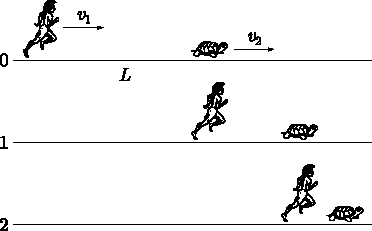
\includegraphics{figure/fig01.02}
    \caption{芝诺时的定义}
    \label{fig:01.02}
\end{figurex}

如图\ref{fig:01.02},阿基里斯和龟在开始时相距为$L$,速度分别为$v_1$及
$v_2$,并且$v_1>v_2$。如果用普通的钟,则阿基里斯将在
\begin{equation}
    t=L/\left(v_1-v_2\right)
    \label{eqn:01.02.01}
\end{equation}
时,赶上龟;当$t>L/\left(v_1-v_2\right)$时,阿基里斯就超过龟了。

图中左边的数字表示的是芝诺时$t'$。当$t'=1$时,阿基里斯到
达龟在0时的出发点;当$t'=2$时,阿基里斯到达龟在1时的出发
点。一般地,当$t'=n$时,阿基里斯到达龟在$t'=n-1$时的位置。
显然,只有当$t'\rightarrow\infty$时,阿基里斯才能逼近龟,对于任何有限的
$t'$,阿基里斯总是落在龟的后面。这就是芝诺的结论。

因此,芝诺断言:“阿基里斯永远也追不上龟。”这里“永
远”的含意是$t'\rightarrow\infty$。,即芝诺时间的无限。

现在我们来讨论普通时$t$与芝诺时$t'$之间的变换关系。不难
验证表\ref{tab:01.02}~给出的两种时间的对应。因此,一般有
{\setlength{\mathindent}{5em}
\begin{equation}
    t=\sum_{n=0}^{t^{\prime}-1} \frac{L}{v_{1}}\left(\frac{v_{2}}{v_{1}}\right)^{n}=\frac{L}{v_{1}-v_{2}}\left[1-\left(\frac{v_{2}}{v_{1}}\right)^{t'}\right]
    \label{eqn:01.02.02}
\end{equation}}%
\clearpage
\noindent 或者\vspace{-1.2em}
\begin{equation}
    t^{\prime}=\frac{1}{\ln \left(v_{2} / v_{1}\right)} \ln \left[1-\left(\frac{v_{1}-v_{2}}{L}\right) t\right]
    \label{eqn:01.02.03}
\end{equation}%
式\eqref{eqn:01.02.02}或式\eqref{eqn:01.02.03}称为芝诺变换。它给出的$t'$与t的关系。在
图\ref{fig:01.03}~中画出。

\begin{table}[!h]
    %\renewcommand\arraystretch{1.6}
    \centering
    \vspace{-0.5em}
    \caption{普通时与芝诺时的关系}
    \label{tab:01.02}
    \begin{tabular*}{\linewidth}{c|>{\qquad}l}
        \toprule
        芝诺时($t'$) & \hspace{7em}普通时($t$) \\
        \midrule
        0       &   0   \\[1.75ex]
        1       &   $\dfrac{L}{v_1}$    \\[1.75ex]
        2       &   $\dfrac{L}{v_1} +\dfrac{L}{v_1}\cdot\dfrac{v_2}{v_1}$ \\[1.75ex]
        \vdots  &   \vdots  \\
        $n$     &   $\dfrac{L}{v_1} + \dfrac{L}{v_1}\cdot\dfrac{v_2}{v_1} + \dots +\dfrac{L}{v_1}\cdot\left(\dfrac{v_2}{v_1}\right)^{n-1} $  \\[1.75ex]
         & $= \displaystyle \sum_{i=0}^{n-1} \frac{L}{v_1}\left(\frac{v_2}{v_1}\right)^i$\\
        \bottomrule
    \end{tabular*}
\end{table}

由图\ref{fig:01.03}~看到,芝诺变换是有奇性的,即当$t=L/\left(v_1-v_2\right)$时,
$t'\rightarrow\infty$。所以,当芝诺时$t'$从零变化到无限时,它只覆盖了普通时
$t$上的一个有限范围,即从零到$ L/\left(v_1-v_2\right) $。

因此,芝诺佯谬之“佯”,是由于芝诺把永远理解为$t'\rightarrow\infty$。
他认为$t'\rightarrow\infty$之后就没有时间了,故$t'\rightarrow\infty$相当于永远。实际上,
从图\ref{fig:01.03}~看到,在芝诺时$ t' $到达无限之后。还是有时间的。但是,
在该范围,即$ t>L/\left(v_1-v_2\right) $,用芝诺钟已经无法度量它们了。简
言之,芝诺的佯谬,来源于芝诺时的局限性,芝诺时不可能度量
阿基里斯追上龟之后的现象。

芝诺佯谬给我们的启示是,时间与时间的度量不同,一种时\clearpage
\begin{wrapfigure}[10]{10}{48mm}
    %\vspace{-0.5em}
    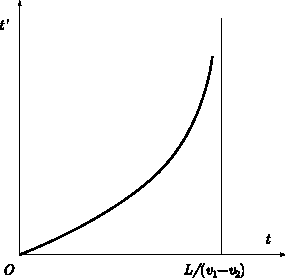
\includegraphics{figure/fig01.03}
    \caption{芝诺时的定义}
    \label{fig:01.03}
    %\vspace{-1.2em}
\end{wrapfigure}
\noindent 间的度量达到无限之后,还是可以有时间的;反之,一种时
间的度量达到无限,从其他的度量看,可能是有限的。

芝诺佯谬还启发我们提出一个更深入的问题,即所谓普通钟
或日常钟是否也具有芝诺钟那种局限性?当日常钟$t$的读数达到
无限之后,是否也还有时间?是否有$t$也无法度量的现象,即在
$t\rightarrow\infty$之外的现象?现代物理学的研究,对这些
问题的回答都是肯定的。
